\section{Assignment 5}

\subsection{Identify the parameters J and D using the LS and the RLS on the DC motors data}

DC motors are characterized by the differential equation:
\begin{equation*}
\tau\dot\omega(t)+\omega(t)=kV(t)
\end{equation*}

that links the applied voltage $V(t)$ to the angular velocity and acceleration of the motor $\omega(t),\dot\omega(t)$ through the constants $k$ and $\tau$. $\tau$ is related to the motor's inertia, while $k$ is related to the motor's torque and electrical constants.

Assuming the motor model is linear, we can estimate $k$ and $\tau$ using Least Squares (LS) regression, which is a method that estimates the vector $\hat\beta$ of parameters that best explains the relation between a set of input vectors $X\in\R^{N\times m}$ to a set of output vectors $Y\in\R^{N\times 1}$. $\hat\beta$ is the parameter vector that minimizes the residual sum of squares (RSS):
\begin{equation*}
\hat\beta = \underset{\beta}{argmin}RSS(\beta)=\underset{\beta}{argmin}(Y-X\beta)^T(Y-X\beta)
\end{equation*}

If $X^TX$ is nonsingular there exists an unique solution given by the normal equations:
\begin{equation*}
\grad_\beta RSS(\beta)=0\iff X^T(Y_X\beta)=0\implies\hat\beta=(X^TX)^{-1}X^TY
\end{equation*}

By expanding the inner products between the vector sets into the sum of the inner products of the vectors that make up the sets and exploiting the matrix inversion lemma to get rid of the matrix inversion, a recursive solution for $\hat\beta$ can be found as:
\begin{align*}
\hat\beta(k)&=\hat\beta(k-1)+K(k)e(k)\;\;\;\;\text{with }\begin{cases}
K(k)&=P(k)x_k^T\\
e(k)&=y_k-x_k\hat\beta(k-1)\\
P(k)&=\frac{1}{\lambda}\left[P(k-1)-\frac{P(k-1)x_k^Tx_kP(k-1)}{\lambda+x_kP(k-1)x_k^T}\right]\end{cases}
\end{align*}

where $\lambda$ is a parameter called forgetting factor which increases the weight of the correction applied to $\hat\beta$ for the most recent samples, which is useful to improve the estimation for time-varying quantities.

Both methods were implemented and tested on data collected from a DC motor modelled in SIMULINK. The $X$ vector set is made up of a set of angular accelerations and velocities obtained by applying a Kalman smoother to the angular position data measured by an encoder, while the $Y$ vector set is made up of the corresponding command voltages. The parameter vector is $\hat\beta=\begin{bmatrix}
k\tau & 1/k
\end{bmatrix}$. LS results are $k=0.7036,\tau=0.2542$ while RLS (with $\lambda=0.975$) results are $k=0.0174,\tau=0.0642$. The corresponding $\hat\beta$ vectors were used to reproject the samples $X$ to obtain an estimation for the voltages $Y$. Figure \ref{fig:ls} shows the resulting estimates against the ground truth.

\begin{figure}[H]
\centering
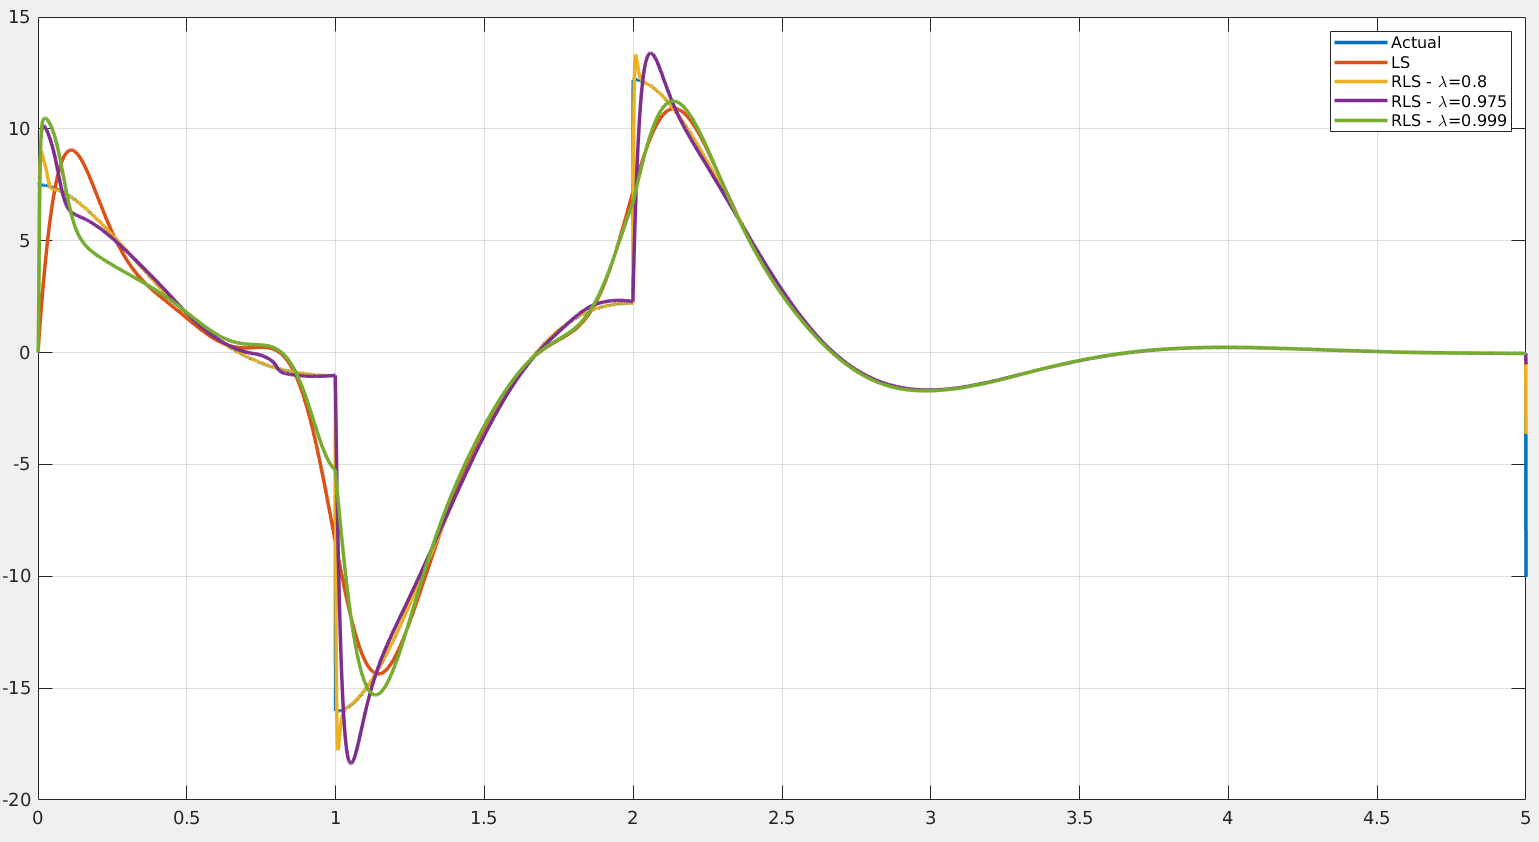
\includegraphics[keepaspectratio,width=0.75\textwidth]{ls}
\caption{Comparison of actual and reprojected voltages}
\label{fig:ls}
\end{figure}

LS performs reasonably well, matching the actual voltages most of the time, but RLS improves greatly the estimation especially around the discontinuities in the actual voltages, showing its capability of accurately tracking time-varying quantities.
Decreasing the value of $\lambda$ results in a model with smaller variance but increased bias towards the ground truth, while increasing it reduces the bias towards the ground truth and increases the variance.